\section{TRNG Implementation}
\label{sec:trng-implementation}

\subsection{Entropy Source}
The entropy source is defined concretely for each device density. For
all 4M (8M) modules, 4-word (32-word) bursts of weight-$D_{\min}$
codewords are identified as the highest entropy rate operation. The
entropy source is derived from a fixed, 256-byte-aligned, contiguous
region in the memory. The region is driven with a fixed repeating
sequence $S_{opt}$, selected from the characterization described in
Section~\ref{sec:trng-optimization}, and latency measurements are
captured for every bursted write. Rather than applying full 256\,B write
transactions with a rotating word-width stride, the runtime sequence
strides the 256\,B region by exactly the burst width in a
non-overlapping manner. This efficient runtime sequence incurs only
$r_t$ cycles on each bitcell, significantly reducing the write pattern
footprint. Because the sequence is wear-leveled within and between
words, repeating complete sequences guarantees that each TRNG access is
wear-leveled. Three 4M and three 8M modules are evaluated as TRNG
sources. One module of each density is placed in a temperature chamber
and heated to $55$\textdegree C. For each module, two fresh (unworn)
256-byte regions are randomly selected, each evaluated as an independent
entropy source.

\begin{figure}[t!]
	\centering
	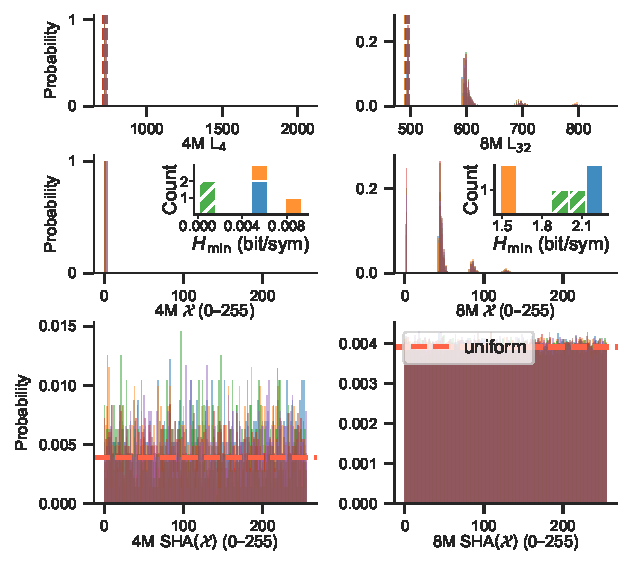
\includegraphics[width=0.9\linewidth]{img/trng_flow_RST_sidebyside.pdf}
	\caption{
		Raw samples (top), symbol mappings and per-region Hmin (middle), and conditioned output (bottom) for 4 fresh 4M (left) and 4 fresh 8M (right) 256B test regions. The $H_{min}$ of each region is colored according the chip in which the region is locate. Two regions are measured at 50\textdegree~C are colored green with a striped texture. NIST 90b reports extremely low $H_{min}$ for all tested regions in the 4M modules, making the required data collection for the NIST-22 and PractRand impractical, while the 8M performs extremely well.
		\label{fig:eval-entropy}
	}
\end{figure}

The characterization in Section~\ref{sec:trng-optimization} demonstrated
that a significant gap in entropy efficiency is closed by burning in the
ReRAM module with 50k full-turnover sequences over the entropy source
region. Profiling before closing this gap substantially underestimates
$H_{\min}$ of the source. A mandatory 50k full-turnover burn-in phase is
therefore applied to each entropy source region before use.

\subsection{Symbol Characterization and Mapping}
After burn-in, each entropy source undergoes a characterization pass in
which $S_{opt}$ is applied 10 times to establish observed minimum and
maximum write latencies. Latencies are then mapped to 1-byte symbols via
a bin assignment scheme. The lowest bin is reserved for underflow
monitoring. The remaining 255 bins are distributed across the observed
latency range with a minimum bin-width equal to the measurement
resolution of the module. If the observed range is narrower than 255
bins at minimum resolution, surplus bins are allocated to capture future
rare high-latency switching events. If the observed range exceeds 255
bins, the bin-width is increased to the smallest integer multiple of the
measurement resolution that accommodates all observed latencies. This
scheme merges adjacent latency values into shared bins and saturates
extreme measurements into the reserved boundary bins, yielding
conservative entropy estimates.

\subsection{Conditioning}
Raw latency samples are conditioned using SHA-256 as a vetted
conditioning component following
SP~800-90B~\cite{sonmez2016recommendation}. Per the standard's vetted
conditioning requirements:
\begin{equation}
	\left\lceil\frac{256 + 64}{H_{\min}}\right\rceil
\end{equation}
1-byte symbols are submitted to the hash
function per 256-bit output block. The 64-bit margin ensures that the
conditioning output is full-entropy with adversarial advantage bounded
by $2^{-64}$. Each symbol is derived from a single write latency
measurement, concatenated with preceding symbols, and hashed to produce
the final output bitstring.
